% $Header: /project/cl/Root/CVS/talks/iowa08/talk.tex,v 1.3 2008/01/31 14:11:37 stump Exp $

\documentclass[10pt]{beamer}

\usepackage{tikz}
\usepackage{pgflibraryarrows}
\usepackage{pgflibraryshapes}
\usepackage{pgfbaseimage}
\usepackage{proof}
\usepackage{url}
\usepackage{code}

\newcommand{\Eq}[0]{\texttt{=}}
\newcommand{\Neq}[0]{\texttt{!=}}
\newcommand{\Qeq}[0]{\stackrel{?}{=}}
\newcommand{\bang}[0]{\texttt{!}}
\newcommand{\quant}[0]{\textit{Quant}}

\newcommand{\To}[0]{\Rightarrow}
\newcommand{\rn}[1]{\textsc{#1}}
\newcommand{\interp}[1]{[ \negthinspace [ #1 ] \negthinspace ]}

\newcommand{\seq}[3]{#1 \vdash #2 : #3}
%\newcommand{\aseq}[3]{ #2 : #3}
\newcommand{\aseq}[3]{ #1 \vdash #3}
%\newcommand{\aaseq}[3]{ #3}
\newcommand{\aaseq}[3]{ #1 \vdash #3}
\newcommand{\abseq}[3]{ #1 \vdash #3}


\mode<presentation>
{
  %\usetheme{Warsaw}
  % or ...

%\usetheme{IowaCity}
\usetheme{Edinburgh}
%\usetheme{Savannah}

%  \setbeamercovered{transparent}
  % or whatever (possibly just delete it)
}


\usepackage[english]{babel}
% or whatever

\usepackage[latin1]{inputenc}
% or whatever

\usepackage{times}
\usepackage[T1]{fontenc}
% Or whatever. Note that the encoding and the font should match. If T1
% does not look nice, try deleting the line with the fontenc.

\title[Resources in Guru]
{Resource Typing in Guru}

\author[Stump, Austin]{Aaron Stump\inst{1} \and Evan Austin\inst{2}}

\institute[Iowa, Kansas]
{
\inst{1}
  Computer Science\\
  The University of Iowa
\and
\inst{2}   Computer Science\\
The University of Kansas
\ \\
\ \\
U.S. National Science Foundation CAREER grant. 
}

% If you have a file called "university-logo-filename.xxx", where xxx
% is a graphic format that can be processed by latex or pdflatex,
% resp., then you can add a logo as follows:

% \pgfdeclareimage[height=0.5cm]{university-logo}{university-logo-filename}
% \logo{\pgfuseimage{university-logo}}



% Delete this, if you do not want the table of contents to pop up at
% the beginning of each subsection:
%\AtBeginSubsection[]
%{
%  \begin{frame}<beamer>
%    \frametitle{Outline}
%    \tableofcontents[currentsection,currentsubsection]
%  \end{frame}
%}


% If you wish to uncover everything in a step-wise fashion, uncomment
% the following command: 

%\beamerdefaultoverlayspecification{<+->}

\begin{document}

\date{\ }

\begin{frame}[plain]
  \titlepage
\end{frame}

\date{PLPV 2010}

\begin{frame}[containsverbatim]
  \frametitle{The \textsc{Guru} Verified-Programming Language}

\begin{itemize}

\item Pure functional language + logical theory. 
\begin{itemize}
\item Includes indexed datatypes, dependent function types.
\item Terms : Types.
\item Proofs : Formulas.
\end{itemize}

\ 

\item Inspired by Coq/CIC, but with some improvements:

\begin{itemize}
\item General recursion for terms.
\begin{itemize}
\item Proofs are still sound.
\item Explicit casts instead of conversion => type equivalence still decidable.
\end{itemize}

\item Annotations dropped for type equivalence.
\begin{itemize}
\item Including types, specificational (``ghost'') data, and proofs.
\item Avoids problems with equality of proofs.
\item Like Implicit Calculus of Constructions (ICC).
\end{itemize}

\item Resource-tracking analysis \textcolor{red}{[new!]}
\end{itemize}
\end{itemize}
\end{frame}

\begin{frame}
\frametitle{The \textsc{Guru} Compiler}
\begin{center}
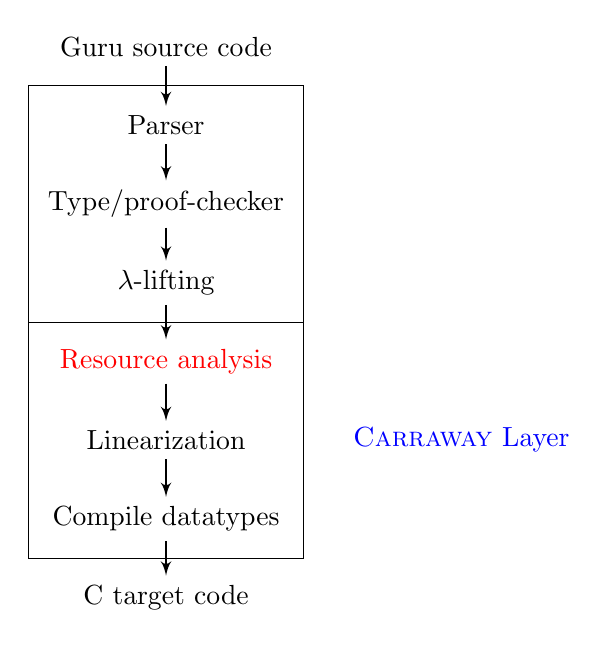
\begin{tikzpicture}
\draw(-1.75,1.5) rectangle +(3.5,3);
\draw(-1.75,-1.5) rectangle +(3.5,3);
\draw(3.75,0) node {\textcolor{blue}{\textsc{Carraway} Layer}};
\draw(0,5)
node(x) {Guru source code};
\draw(0,4)
node(a) {Parser};
\draw(0,3)
node(b) {Type/proof-checker};
\draw(0,2)
node(c) {$\lambda$-lifting};
\draw(0,1)
node(d) {\textcolor{red}{Resource analysis}};
\draw(0,0)
node(e) {Linearization};
\draw(0,-1)
node(f) {Compile datatypes};
\draw(0,-2)
node(g) {C target code};
\draw[-latex',black,thick](x.south) -- (a.north);
\draw[-latex',black,thick](a.south) -- (b.north);
\draw[-latex',black,thick](b.south) -- (c.north);
\draw[-latex',black,thick](c.south) -- (d.north);
\draw[-latex',black,thick](d.south) -- (e.north);
\draw[-latex',black,thick](e.south) -- (f.north);
\draw[-latex',black,thick](f.south) -- (g.north);
\end{tikzpicture}
\end{center}
\end{frame}

\begin{frame}
\frametitle{Functional Modeling for Imperative Abstractions}

\begin{itemize}
\item I/O, mutable arrays, cyclic structures, etc.
\item Do not fit well into pure FP.
\item Approach: functional modeling. \footnote{Cf. ``Beauty in the Beast'' \textcolor{blue}{[Swierstra and Altenkirch 2007]}}
\begin{itemize}
\item Define a pure functional model (e.g., \texttt{<list A n>} for arrays).
\item Model is faithful, but slow.
\item Use during reasoning.
\item Replace with imperative code during compilation.
\item Use \emph{linear} types (alternatively, monads) to keep in synch.
\end{itemize}
\item Combining dependent and linear typing is powerful.
\begin{itemize}
\item Cf. ``Safe Programming with Pointers through Stateful Views'' \textcolor{blue}{[Zhu,Xi 2005]}.
\item Also, ``End-to-end Verification of Security Enforcement is Fine'' \textcolor{blue}{[Swamy,Chen,Chugh 2009]}.
\end{itemize}
\end{itemize}
\end{frame}

\begin{frame}
\frametitle{A Resource Typing Framework}
\begin{itemize}
\item Idea: explore resource management with a framework.
\item Framework implements concepts of resource, subresource.
\item Different resource abstractions then defined:

\ 

\textcolor{purple}{reference-counted data}\ \ \ \ \ \ \ \ \textcolor{orange}{unique references}


\ 

\ \ \ \textcolor{brown}{heap abstractions} \ \ \ \textcolor{green}{read-only views}

\ 

\item On top of these, build data abstractions:

\begin{itemize}
\item Mutable array abstractions.
\item Aliased data structures (e.g., FIFO queues). 
\end{itemize}

\end{itemize}
\end{frame}

\begin{frame}
  \frametitle{A Framework for Resources}

\begin{itemize}

\item Fundamental ideas:

\begin{enumerate}
\item A resource can only be used by one entity at a time.
\item A resource can be temporarily decomposed into subresources.
\end{enumerate}

\item Resource abstraction defined by \emph{primitives}:

\begin{itemize}
\item a trusted resource type,
\item a functional model in \textsc{Guru},
\item trusted C code implementing the primitive.
\end{itemize}

\item Resource analysis:
\begin{itemize}
\item Check linearity conditions (used exactly once).
\item Track subresource relationships.
\item Enforce \emph{consumption annotations} on input variables:
\begin{itemize}
\item (default)\ \ -- \ \ consume exactly once.
\item \textbf{\^{\ }}\ \ -- \ \  consume but do not return.
\item \textbf{!} \ \ -- \ \  do not consume.
\end{itemize}
\end{itemize}

\end{itemize}

\end{frame}

\begin{frame}
\frametitle{Subresources}

\begin{itemize}
\item ``Deathly Hallows'' as subresource of Harry Potter boxed set.
\item Sublist \texttt{l'} as a subresource of \texttt{(cons x l')}.
\item Subresource relationship based on type \texttt{<R x>}:
\begin{itemize}
\item \texttt{x:R} \ \ -- \ \ x has resource type R.
\item \texttt{y:<R' x>} \ \ -- \ \  y has resource type R', and is a subresource of x.
\end{itemize}

\item Cannot consume \texttt{x} until all subresources have been consumed.

\end{itemize}

\end{frame}

\begin{frame}[containsverbatim]
\frametitle{Resource Abstraction: Reference-Counted Data}
{
\footnotesize
\begin{verbatim}
ResourceType unowned [...].

Define primitive inc
 : Fun(spec A:type)(! #unowned y:A).#unowned A
 := fun(A:type)(y:A).y 
<<END
  inline void *ginc(void *y) { [...] }
END.

Define primitive dec
 : Fun(A:type)(^#unowned y:A).void
 := fun(A:type)(y:A).voidi 
<<END
  void gdec(int A, void *r) { [...] }
END.
\end{verbatim}
}

All inductive (tree-like) data are reference-counted.
\end{frame}


\begin{frame}[containsverbatim]
\frametitle{Resource Abstraction: Owned References}
\footnotesize
\begin{verbatim}
ResourceType owned affine.

Define primitive inspect
 : Fun(spec A:type)(!#unowned x:A).#<owned x> A 
 := fun(A:type)(x:A).x
<<END
  #define ginspect(x) x
END.
\end{verbatim}

\begin{itemize}
\item Cannot consume \texttt{x:A} before \texttt{y:\#<owned x> A}.
\item This \texttt{y} is \emph{pinning} \texttt{x}.
\item So no \texttt{inc},\texttt{dec} required.
\item => improved performance, still memory safe.
\end{itemize}

\end{frame}

\begin{frame}[containsverbatim]
\frametitle{Initializing Subdata in \texttt{match}-cases}
\begin{itemize}
\item \texttt{Init}-function defined as part of resource abstraction.
\item Suppose matching on \texttt{x:r}, subdatum \texttt{y:r'}.
\item \texttt{Init}-function for \texttt{r-r'} initializes \texttt{y}.

{\footnotesize
\begin{verbatim}
Init ginit_unowned_unowned(#unowned x)(#unowned y).#unowned 
<<END
  inline void *ginit_unowned_unowned(int A,void *x,void *y) {
    ginc(y);
    return y;
  }
END.

Init ginit_owned_unowned(#owned x)(#unowned y).#<owned x> <<END
  #define ginit_owned_unowned(A,x,y) y
END.
\end{verbatim}
}

\item Compressing chains of ownership:
\[
\infer{\texttt{@ t:<r z>}}{\texttt{t:<r y>} & \texttt{y:<r' z>}}
\]

\end{itemize}
\end{frame}

\begin{frame}
\frametitle{Data Abstraction: Word-Indexed Mutable Arrays}

\begin{itemize}
\item Type: \texttt{<warray A N L>}.
\item Resource type: \texttt{unique}.
\begin{itemize}
\item \texttt{A} is type of elements.
\item \texttt{N} is length of array.
\item \texttt{L} is list of initialized locations.
\end{itemize}

\item \texttt{(new\_array A N) : <warray A N []>}.

\item Writing to index \texttt{i}: 
\begin{itemize}
\item requires proof: \texttt{i < N}.
\item functional model: consume old array, produce updated one.
\item imperative implementation: just do the assignment.
\item array's type changes:  \texttt{<warray A N i::L>}.
\end{itemize}

\item Reading from index \texttt{i}:
\begin{itemize}
\item does not consume array.
\item requires proof: $\texttt{i}\in\texttt{L}$.
\end{itemize}
\end{itemize}
\end{frame}

\begin{frame}
\frametitle{Example: FIFO Queues}

\begin{itemize}
\item Mutable singly-linked list, with direct pointer to end.
\item \textbf{Aliasing!}
\item \textsc{Guru} approach: \emph{heaplets} (part of heap).

\ 

{\small
\begin{tabular}{|l|l|l|}
\hline
Type & Functional Model & Imperative Implementation \\
\hline
\texttt{<heaplet A I>} & list of aliased values & nothing\\
\texttt{<alias I>} & index into heaplet \texttt{I} & reference-counted pointer\\
\hline
\end{tabular}}

\ 

\ 

\item Unverified queue:
\begin{itemize}
\item Just memory safety.
\item 138 lines total (6 lines proof).
\end{itemize}

\ 

\item Verified queue:
\begin{itemize}
\item Prove that \texttt{qin}-node has no next-pointer.
\item Requires reasoning about aliases.
\item 310 lines total (178 lines proof).
\end{itemize}

\end{itemize}
\end{frame}

\begin{frame}
\frametitle{Garbage Collection, Or Lack Thereof}
\begin{itemize}
\item Garbage collection has led to great productivity gains...
\item ... but hurts performance generally.
\item No continuum: either all GC (\textcolor{orange}{slow}) or no GC (\textcolor{purple}{unsafe}).
\item \textsc{Guru} does not use GC.
\begin{itemize}
\item Resource abstractions are memory safe.
\item But \texttt{heaplet} can leak memory for cyclic structures.
\end{itemize}
\item A perfect world might provide:
\begin{itemize}
\item GC'ed regions for productivity.
\item Heavier abstractions for safety without GC.
\begin{itemize}
\item E.g., \emph{compile-time} reference counting.
\item Significant verification burden.
\end{itemize}
\item Key: ability to choose which is more appropriate.
\end{itemize}
\end{itemize}
\end{frame}

\begin{frame}
\frametitle{Empirical Comparison}
Benchmark 1: In array storing $[0,2^{20})$, do binary search for each element.

\ 

Benchmark 2: push all words in ``War and Peace'' through 2 queues.

\ 

\ 


{\footnotesize
\begin{tabular}{lr}
\begin{tabular}{| l | l | l |}
\hline
\multicolumn{3}{|c|}{Mutable Array Test} \\
\hline
Language & Time & Binary \\
\hline
\textcolor{red}{\textsc{Haskell}} & \textcolor{red}{1.18 s} & 581K\\
\textsc{Haskell} (No GC) & 0.49 s & \ \\
\textcolor{red}{\textsc{OCaml}} & \textcolor{red}{0.61 s}  & 131K\\
\textsc{OCaml} (No GC) & 0.54 s & \ \\
\textcolor{red}{\textsc{Guru}} & \textcolor{red}{0.42 s} & 37K\\
\hline
\end{tabular}
&
\begin{tabular}{| l | l | l |}
\hline
\multicolumn{3}{|c|}{Queue Test} \\
\hline
Language & Time & Binary \\
\hline
\textcolor{red}{\textsc{Haskell}} & \textcolor{red}{1.08 s} & 614K\\
\textsc{Haskell} (No GC) & 0.53 s & \ \\
\textcolor{red}{\textsc{OCaml}} & \textcolor{red}{0.66 s} & 132K\\
\textsc{OCaml} (No GC) & 0.37 s & \ \\
\textcolor{red}{\textsc{Guru}} & \textcolor{red}{0.60 s} & 37K\\
\hline
\end{tabular}
\end{tabular}
}

\ 

\ 

\ \ \ \ \ \ \ \ \ \ \ \ \ \ \ \ \ \ \ \ \ \ \ \ \ \ \ \ \ \ \ {\footnotesize
\begin{tabular}{r}
Compilers: \texttt{ghc 6.10.4, ocamlopt 3.11.1, gcc 4.3.3} \\

Machine: \texttt{2.67Ghz Intel Xeon, 8 GB mem, Linux 2.6.18}
\end{tabular}}

\end{frame}

\begin{frame}
\frametitle{Future Directions}

\begin{itemize}
\item Better abstractions for aliased structures.

\item Realistic applications.

\begin{itemize}
\item \texttt{versat}: verified modern SAT solver.
\begin{itemize}
\item Complex code, uses mutable state.
\item Not too large.
\item Simple spec.: learned clauses derivable by resolution from input clauses.
\end{itemize}
\end{itemize}

\item Meta-theoretic work.

\item To learn more:

\begin{center}
\Large
\textcolor{blue}{\url{www.guru-lang.org}}
\end{center}

\ 

``Verified Programming in Guru'' book.

\end{itemize}

\end{frame}

\end{document}

